%!TEX output_directory = aux

\documentclass[11pt]{article}

\usepackage[english]{babel}

% ---- FONT & MICROTYPOGRAPHY ----
\usepackage[utf8]{inputenc}
\usepackage[T1]{fontenc}
\usepackage{microtype}
\usepackage{moresize}

% ---- FORMATTING ----
\usepackage{csquotes,textcase,xspace}

% ---- PAGE LAYOUT ----
\usepackage{geometry}
\geometry{top=2.5cm,bottom=2cm,inner=2cm,outer=2cm,footnotesep=7mm plus 4pt minus 4pt}
\usepackage{setspace}
\setstretch{1.1}

% ---- GRAPHIQUE ----
\usepackage{graphicx}
\usepackage{xcolor}
\usepackage[font=small,labelfont=bf,labelsep=space]{caption}
\usepackage{subfigure}
\captionsetup{width=0.9\textwidth,font={small,stretch=1.1}}
\addto\captionsenglish{\renewcommand{\figurename}{Fig.}}
\addto\captionsenglish{\renewcommand{\tablename}{Tab.}}
\definecolor{JoliBleu}{rgb}{0,0.55,0.55}
\definecolor{JoliVert}{rgb}{0.15,0.6,0}
\definecolor{JoliRouge}{rgb}{0.86,0.08,0}
\definecolor{JoliJaune}{rgb}{1,0.75,0}
\definecolor{JoliGris}{rgb}{0.52,0.52,0.51}
\definecolor{myblue}{RGB}{26, 77, 116}
\definecolor{myorange}{RGB}{181, 116, 30}
\definecolor{mydarkorange}{RGB}{166, 88, 0}
\definecolor{mygreen}{RGB}{21, 124, 80}
\definecolor{myblack}{RGB}{43, 65, 82}
\definecolor{myred}{rgb}{0.5, 0.0, 0.13}

% ---- SECTIONING ----
\usepackage{titlesec}
\titleformat{\section}[block]{\Large\boldmath\bfseries}{\thesection}{1em}{}
\titleformat{\subsection}[block]{\large\boldmath\bfseries}{\thesubsection}{0.5em}{}
\usepackage{appendix}
\renewcommand{\setthesection}{\Alph{section}}
\renewcommand{\restoreapp}{}
\makeatletter
\renewcommand{\theequation}{\thesection.\arabic{equation}}
\@addtoreset{equation}{section}
\makeatother

% ---- FOOTERS HEADERS ----
\usepackage[bottom]{footmisc}
\usepackage{fancyhdr}

% ---- TABLE OF CONTENTS ----
\usepackage{titletoc}
\setcounter{tocdepth}{3}

% ---- BIBLIOGRAPHY ----
\usepackage[nosort]{cite}
\bibliographystyle{JHEP}
\newcommand{\eprint}[1]{{\href{http://arxiv.org/abs/#1}{\texttt{[#1]}}}}
\newcommand{\eprintN}[1]{{\href{http://arxiv.org/abs/#1}{\texttt{#1 [hep-th]}}}}
\newcommand{\doi}[2]{\href{http://dx.doi.org/#2}{#1}}

% ---- HYPER REF ----
\usepackage{hyperref}
\hypersetup{colorlinks=true,
        pdfstartview=FitV,
        linkcolor= mydarkorange,
        citecolor= mydarkorange, 
        urlcolor= JoliGris!60!black,
        hypertexnames=false,
        linktoc=page}

% ---- TIKZ ----
\usepackage{tikz}
\usetikzlibrary{calc}

% ---- MATHS ----
\usepackage{amsmath,amssymb,amsfonts,dsfont}
\usepackage{mathrsfs}
\usepackage{physics}
\usepackage{ytableau}
\ytableausetup{boxsize=1.1em,centertableaux}
\usepackage{stmaryrd}
\usepackage{nicefrac}
\allowdisplaybreaks[1]
% \usepackage{bbold}
\usepackage{cases}
\usepackage{bm}
\usepackage{bbm}

% ---- TABLES ----
\usepackage{multirow}
\usepackage{booktabs}
\usepackage{pdflscape}
\usepackage{array}
\usepackage{arydshln}

% ---- ENUMERATION ----
\usepackage[shortlabels]{enumitem}

% ---- MATHS COMMANDS ----
\newcommand{\A}{\ensuremath{\mathcal{A}}\xspace}
\newcommand{\F}{\ensuremath{\mathcal{F}}\xspace}
\renewcommand{\H}{\ensuremath{\mathcal{H}}\xspace}
\newcommand{\M}{\ensuremath{\mathcal{M}}\xspace}
\renewcommand{\P}{\ensuremath{\mathcal{P}}\xspace}
\newcommand{\J}{\ensuremath{\mathcal{J}}\xspace}
\renewcommand{\d}{\ensuremath{\mathrm{d}}\xspace}
\renewcommand{\H}{\ensuremath{\mathcal{H}}\xspace}
\newcommand{\SO}{\ensuremath{\mathrm{SO}}\xspace}
\renewcommand{\O}{\ensuremath{\mathrm{O}}\xspace}
\newcommand{\SL}{\ensuremath{\mathrm{SL}}\xspace}
\newcommand{\Odd}{\ensuremath{\mathrm{O}(d,d)}\xspace}
\newcommand{\odd}{\ensuremath{\mathfrak{o}(d,d)}\xspace}
\renewcommand{\Tr}[1]{\ensuremath{\mathrm{Tr}\left(#1\right)}\xspace}
\newcommand{\vol}{{\,\rm vol}}
\def\sst#1{{\scriptscriptstyle #1}}


\def\0{{\sst{(0)}}}
\def\1{{\sst{(1)}}}
\def\2{{\sst{(2)}}}
\def\3{{\sst{(3)}}}
\def\4{{\sst{(4)}}}
\def\5{{\sst{(5)}}}
\def\6{{\sst{(6)}}}
\def\7{{\sst{(7)}}}
\def\8{{\sst{(8)}}}

\newcommand{\be}{\begin{equation}}
\newcommand{\ee}{\end{equation}}

% ---- COMMENTS ----
\newcommand{\ce}[1]{\marginpar{\parbox{\marginparwidth}{\boldmath $\Longleftarrow$}}{\boldmath\bfseries (ce: #1)}}
\newcommand{\gl}[1]{\marginpar{\parbox{\marginparwidth}{\boldmath $\Longleftarrow$}}{\boldmath\bfseries (gl: #1)}}




%%%%%%%%%%%%%%%%%%%%%%%%%%%%%%%%%%
%%%%%%%%%%%%%%%%%%%%%%%%%%%%%%%%%%


\begin{document}

\begin{titlepage}



\begin{flushright}

MI-HET-??? \\
\today
\end{flushright}


\vspace{25pt}

   
   \begin{center}
   \baselineskip=16pt


   \begin{Large}

\mbox{ \bfseries \boldmath  Notes: Machine learning flat directions}
   \end{Large}


   		
\vspace{25pt}
		

{\large  Bastien Duboeuf$^{1}$, Camille Eloy$^{1}$ \,and\, Gabriel Larios$^{2}$}
		
\vspace{25pt}
		
		
	\begin{small}

	{\it $^{1}$ ENS de Lyon, CNRS, LPENSL, UMR5672,\\ 69342, Lyon cedex 07, France}  \\


	\vspace{10pt}
	
	{\it $^{2}$ Mitchell Institute for Fundamental Physics and Astronomy, \\
	Texas A\&M University, College Station, TX, 77843, USA}     \\
		
	\end{small}
		

\vskip 50pt

\end{center}


\begin{center}
\textbf{Abstract}
\end{center}


\begin{quote}

...

\end{quote}

\vfill

\end{titlepage}


\tableofcontents



\section{Introduction}

\section{Supergravity setup}
\begin{itemize}[label=\textbullet]
	\item Context: 6d ${\rm AdS}_{3}\times S^{3}$, truncation to 3d, potential, conformal manifold.
	\item Choice of truncation from 32 to 13 to 5 variables.
\end{itemize}

\paragraph{Potential}
The 22 scalars of the theory can be parametrised by ($22 = 32 - 10$, with 10 scalars gauge fixed using translations in the gauge group)
\begin{itemize}[label=\textbullet]
	\item $m = \nu\nu^{T}\in{\rm GL}(3,\mathbb{R})$ parametrizing the coset ${\rm GL}(3,\mathbb{R})/{\rm SO}(3)$,
	\item $\phi$ a $3\times3$ antisymmetric matrix,
	\item $\xi$ a $3\times4$ matrix, and $\xi^{2} = \xi \xi^{T}$,
	\item a dilaton $\tilde{\varphi}$.
\end{itemize}
We can further restrict ourselves to a set of 13 scalars (see ref.~\cite{Eloy:2021fhc}), with
\begin{equation}
	\begin{aligned}
		\xi &= \begin{pmatrix}
					0 & 0 & 0 & x_{1} \\
					0 & 0 & 0 & x_{2} \\
					0 & 0 & 0 & x_{3}
				\end{pmatrix},
		\quad
		\phi = \begin{pmatrix}
					0 & x_{4} & x_{5} \\
					-x_{4} & 0 & x_{6} \\
					-x_{5} & -x_{6} & 0
				\end{pmatrix},
		\quad
		\tilde{\varphi} = x_{13} \\[5pt]
		\nu &= e^{(6\,x_{7}+3\,x_{8}+\sqrt{3}\,x_{9})/6}
				\begin{pmatrix}
					1 & \frac{x_{10}}{\sqrt{2}} & \frac{x_{11}}{\sqrt{2}} + \frac{x_{10}x_{12}}{4} \\
					0 & e^{-x_{8}} & \frac{e^{-x_{8}}\,x_{12}}{\sqrt{2}} \\
					0 & 0 & e^{-(x_{8}+\sqrt{3}\,x_{9})/2}
				\end{pmatrix}.
	\end{aligned}
\end{equation}
Scalar potential from ref.~\cite{Eloy:2021fhc}:
%
\begin{equation} \label{eq:scalarpotential}
	\begin{aligned}
 		V & = 4\,e^{-4\tilde\varphi}+2\,e^{-2\tilde\varphi}\Big[-\tr\left(m+m^{-1}\right)+\tr\left(\phi m^{-1}\phi\right) -2\,\tr\left(\phi m^{-1}\xi^{2}\right)-2\,\tr\left(\xi^{2}\right)\\
 		&\qquad\quad-\tr\left(\xi^{2}m^{-1}\xi^{2}\right)  +\frac{1}{2}\,\det\left(m^{-1}\right)\left(1-\tr\left(\phi^{2}\right)-\tr\left(\xi^{4}\right)+\tr\left(\xi^{2}\right)^{2}\right) \\
 		&\qquad\quad +\frac{1}{2}\,{\rm T}\left(m^{-1}(\xi^{2}-\phi),(\xi^{2}+\phi)m^{-1},m+(\xi^{2}+\phi)m^{-1}(\xi^{2}-\phi)+2\,\xi^{2}\right)\\
 		&\qquad\quad +\frac{1}{4}\,{\rm T}\left(m^{-1},m+(\xi^{2}+\phi)m^{-1}(\xi^{2}-\phi)+2\,\xi^{2},m+(\xi^{2}+\phi)m^{-1}(\xi^{2}-\phi)+2\,\xi^{2}\right)\Big], 
 	\end{aligned}
\end{equation}
where ${\rm T}\left(A,B,C\right)=\varepsilon_{mnp}\,\varepsilon_{qrs}\,A^{mq}B^{nr}C^{ps}$.

As a first simplified example we have considered only the parameters $x_{1}, x_{2}, x_{4}, x_{8}$ and $x_{10}$. The potential~\eqref{eq:scalarpotential} becomes
\begin{equation} \label{eq:scalarpotential124810}
	\begin{aligned}
		V &= \frac{1}{8}\, e^{-2\,x_{8}} \bigg[4 + 4\,x_{1}^4 + e^{4\,x_{8}} \big(2 + x_{10}^2\big)^2 \big(1 + x_{2}^4\big)\\
		  & \quad\qquad\qquad - 4\,e^{3\,x_{8}}\,\big(2 + x_{10}^2\big) \Big(2 - x_{1}^2 + \sqrt{2}\,x_{1} x_{10} x_{2}^3 + x_{2}^4 + 
      			2\,x_{1} x_{2} x_{4} + x_{4}^2 - x_{2}^2 \big(1 - x_{1}^2 + x_{4}^2\big)\Big)\\
        & \quad\qquad\qquad - 8\,e^{x_{8}}\,\Big(2 + x_{1}^4 + \sqrt{2}\,x_{1}^3 x_{10} x_{2} - x_{2}^2 - 2\,x_{1} x_{2} x_{4} + 
      			x_{4}^2 - x_{1}^2 \big(1 - x_{2}^2 + x_{4}^2\big)\Big)\\
        & \quad\qquad\qquad + 4\,e^{2\,x_{8}}\,\Big(2 - 4\,x_{1}^2 + x_{1}^4 - 4\,x_{2}^2 + 4\,x_{1}^2 x_{2}^2 + x_{2}^4
        			+ x_{10}^2\big(1 + 3\,x_{1}^2 x_{2}^2\big) + 4\,x_{4}^2 + x_{4}^4\Big)\\
        & \quad\qquad\qquad + 8\sqrt{2}\,x_{10}\,e^{2\,x_{8}}\,\Big(x_{1}^3 x_{2} + x_{1}^2 x_{4} - x_{2}^2 x_{4} + x_{1} \big(x_{2}^3 - x_{2} x_{4}^2\big)\Big)\bigg].
	\end{aligned}
\end{equation}
\ce{Change notation to keep $x$ for the polynomial variables?}

\ce{Discuss here why we need numerical methods: to complicated for mathematica to simplify the gradient.}

\section{Numerical analysis}
	\subsection{Gradient descent and local analysis}
		\paragraph{Gradient descent: implementation, sampling, time needed, loss}
		In order to look for flat direction in this potential, we will use numerical tools. The path we will follow is the following : first we will sample the underlying manifold, then we will use numerical tools to exctract analytics information on this cloud of points. Therefore the first step is to sample the manifold. To do so, we choose to do a basic gradient descent. We start by randomly uniformy initializing points in an hypercube of length $[-2,2]$. This will be important latter to have points which are not only in $[-1,1]$. We choose to have $10^5$ points. For this example. This number is motivated by the dimensionality of our problem. If all possible directions are going to be populated, and if wen want $\mathcal{O}(10)$ points in each direction, then we need  $\mathcal{O}(10^5)$ points. As the true internal dimension of the manifold is lesser or equal than 5, this number provides an upper bound for the number of points needed to sufficiently sample the manifold.  We then perfom a gradient descent on the point using the automatic differentiation method of tensorflow. For the loss function, we use 
		\begin{equation}
			\mathcal{L} = \sum_{i = 1}^{n_{points}} |\nabla V(\vec{x}^{\,i})|^2
		\end{equation}
		with $\vec{x}^{\,i} = (x^i_1,x^i_2,x^i_4,x^i_8,x^i_{10})$ are the data points. We choose to use the Adam optimizer and use a learning rate of $10^{-2}$. We run the gradient descent for $10000$ epochs to make sure of convergence. 
%		\begin{figure}
%			\includegraphics[scale = 0.5]{imagefile} % add loss history 
%		\end{figure}
		As a first visualisation, we show a triangular plot of the data in Fig. \ref{triangular_plot_1_2_4_8_10}. This shows all possible $2d$ projections of the data as well as the $1d$ histograms of the data after the gradient descent. 
		\begin{figure}[t]
			\centering
			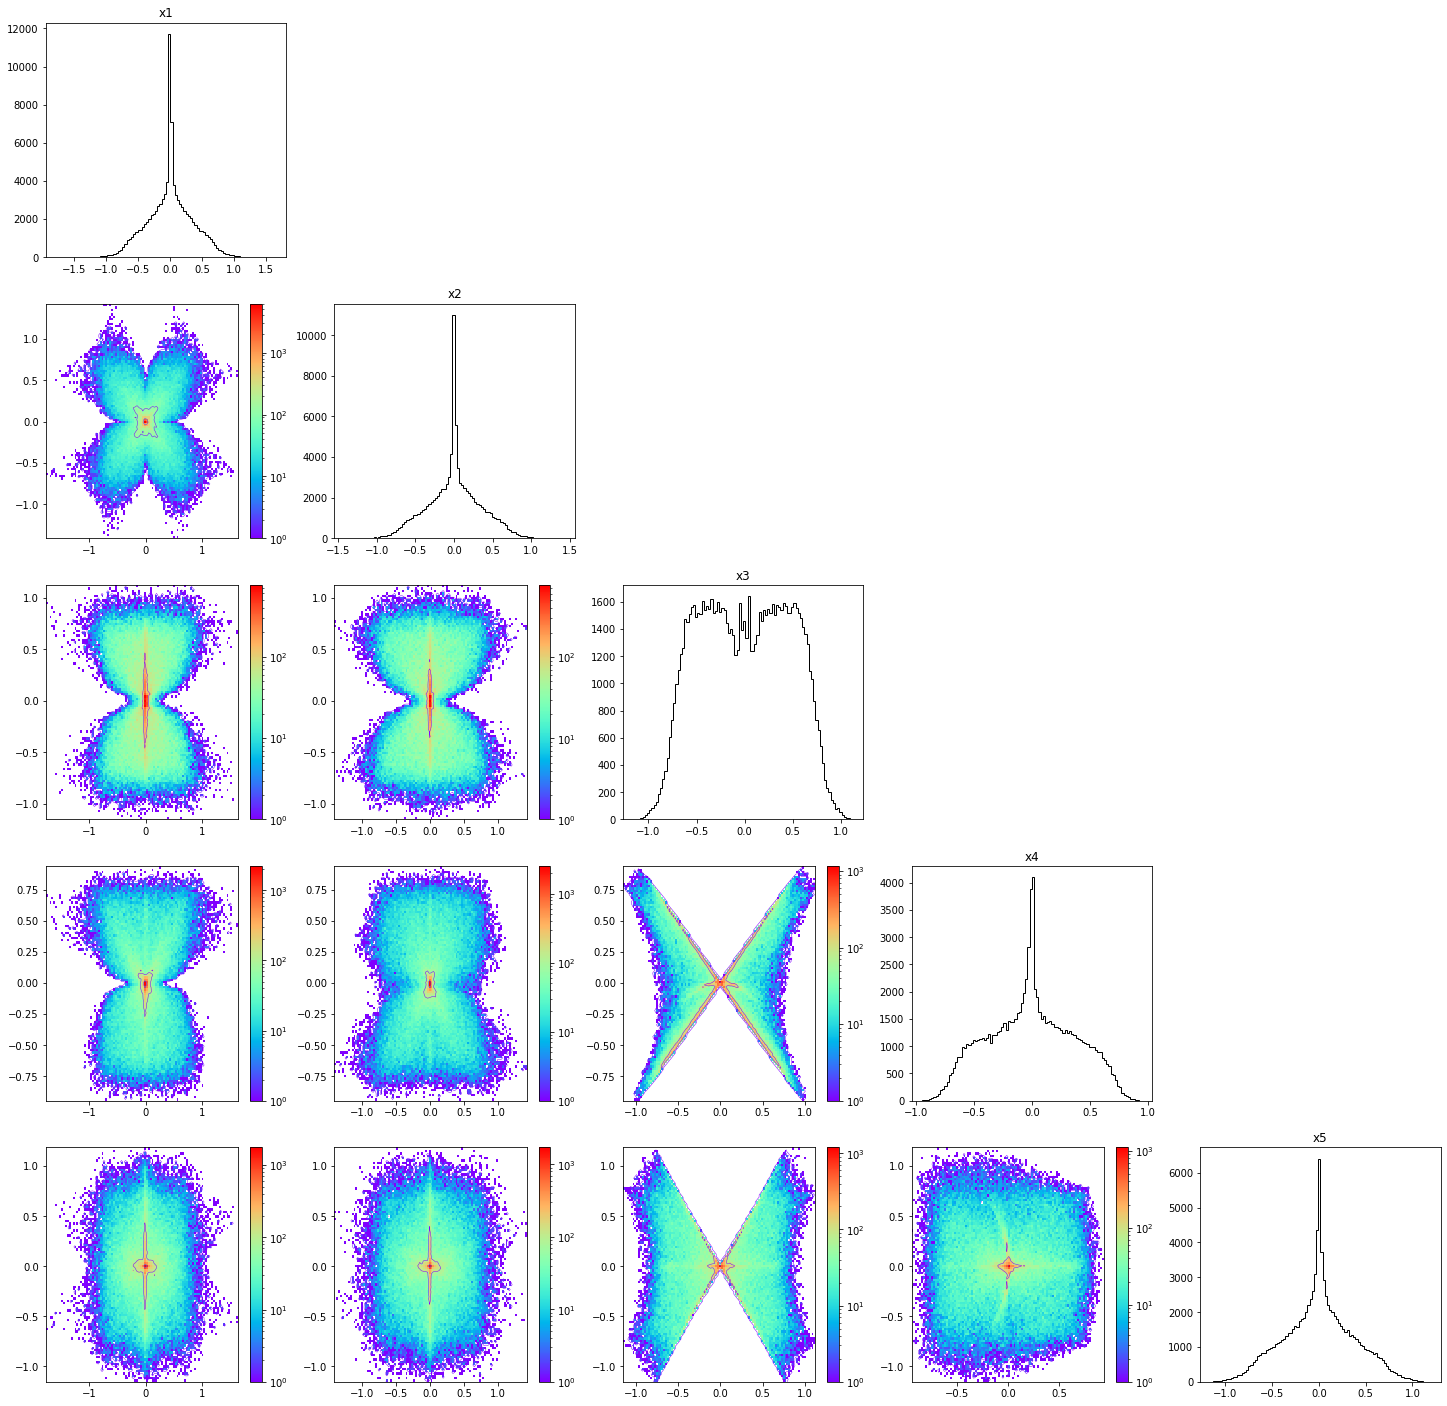
\includegraphics[scale = 0.25]{Figures/triangular_plot_1_2_4_8_10.png} %names need to be changed.
			\caption{Triangular plot showing $2d$ projections and $1d$ histograms of the data after the gradient descent}
			\label{triangular_plot_1_2_4_8_10}
		\end{figure}
		
		Comments :
		\begin{enumerate}
			\item We see some non trivial correlation between the data. Note however that some features we see can be caused by the fact that some places may be greater basin of attractions (this is for example what happend in the $x_1/x_2$ plot). However, the structure we see in the $x_4/x_8$ or $x_4/x_{10}$ is a remnant of true features of the manifold
			\item All directions seems to be well populated 
			\item A great majority of the points fall in the $\vec{0}$ point. This is not too surprising. This just means that the round sphere solution has a greater basin of attraction. Even so, those points are going to be sufficiently good for the rest of the analysis, and we do not try to move the points along flat directions (to depopulate the origin et repopulate the rest).
		\end{enumerate}

		\paragraph{Local PCA: graphs of number of patches with given local dimension, and with varying size of local patch, discuss optimal patch size (we want at least fex points in each direction)}
		
		Once the gradient descent is done and we sampled the flat direction, it remains to determine what is the underlying manifolds. We would like to obtain some analytics expression for this, not only a numerical solution. Before proceeding to any sort of symbolic regression and look for such an analytic expression, there is a few things we can do to gain so understanding on the data, such as determining the dimensionality of the manifold, and wheter it a one piece or several pieces manifolds (like 2 intersecting hyperplane or so). To do so, we run a local Principal Component Analysis (PCA) algorithm. For each point, we select the $k$ nearest neighboors, and we run a PCA analysis on thos points. This allows to determine how many directions are needed to explain a given percentage of the spreding of the data, call it $\epsilon$. In other words, this allows to determine what is the local dimension around each point. We ran such an algorithm for a number of $k$ nearest neighboors equal to $[5,10,20,50,100]$, and for $\epsilon = 0.99$. The results are shown in \ref{local_pca}.
		\begin{figure}
			\centering
			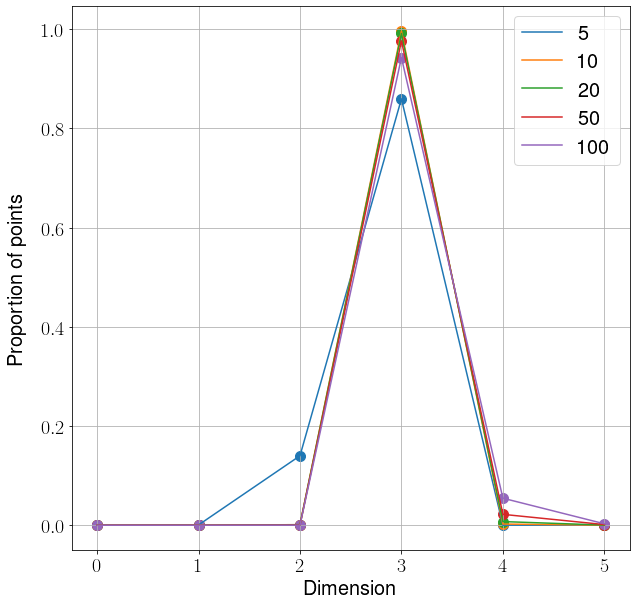
\includegraphics[scale=0.5]{Figures/Local_PCA.png}
			\caption{Results of the local PCA analysis. On the $x$-axis is the dimension found by the algorithm, and on the $y$-axis the proportion of points. The different curves are for different $k$-nearest neighboors.}
			\label{local_pca}
		\end{figure} 
		
		We see that, for every choice of nearest neighboor, a peak at $d=3$, which indicates an underlying dimension of 3 for the manifold. We also see that for $k=5$, that a number a point seems to indicate a dimensionality of 2. However, if the dimension is indeed 3, then 5 points may not be enough to sufficiently populate the three directions, explaining the failure of the algorithm to find 3. We also see that for $k\le20$, that there is more and more points indicating a dimension equals to 4 or 5. This can be explained by the fact that we increasing the number of neighboors, we are doing a rougher coarse graining, loosing information on the localilty. A too large number of neighboors implies including points which are not really local anymore, artificially increasing the local dimension. We conclude that the dimension of the manifold we are looking at is 3. 
		
		\paragraph{Clusteting: HDBScan (only parameter: minimal number of points in a cluster), and graphs of 3d slices of the 5d space}
		Something that might happen, is that we have several manifolds of dimesion 3, and the dimension 4 points we saw above are actually the intersection of those manifolds. If we indeed picture the intersection of two lines, then at the intersection point, the local dimension found by the previous algorithm should be 2. To exclude such a scenario, we run a clustering algorithm, based on local density. For this, we use the HDBSAN algorithm. (details on how it works?). We choose a minimal cluster size of 10 points. Out of the 100000, the algorithm finds 3 cluster : one on dimension 10, one of dimension 91747 and a last one of dimension 6849 (not a total of 100000?? Clustering only on the point with 3d neighbourhood to avoid intersections). The last cluster are just the points that the algorithm did not managed to fit into any cluster. For the first one, we interpret it as some fluctuation in our data, making some region of different density as the other, but we do not believe this is some real result, more an artefact. Therefore, what the algorithm tells us, is that there seems to be on cluster with more than $90\%$ of the data. We show on \ref{3dplots} three-dimensional projections of the data. 
		
		\begin{figure}
			\centering
			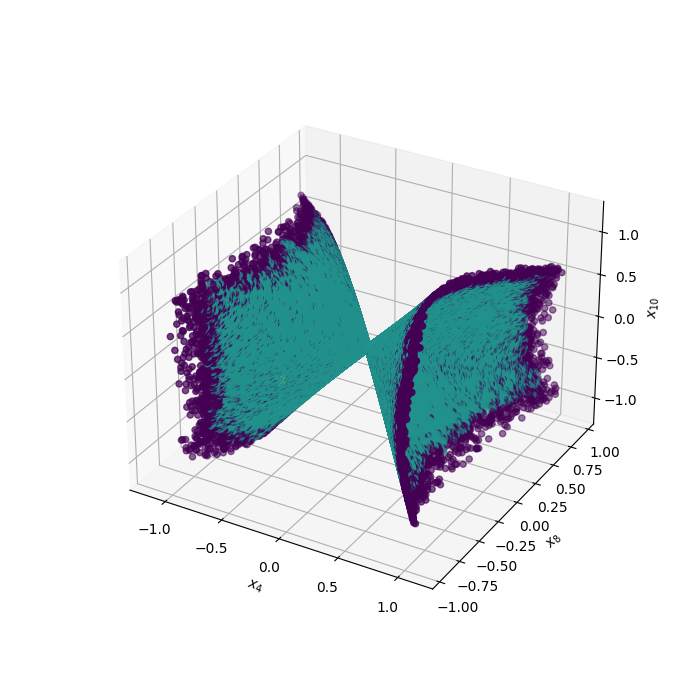
\includegraphics[scale=0.4]{Figures/3d_plot_x4_x8_x10.png}
			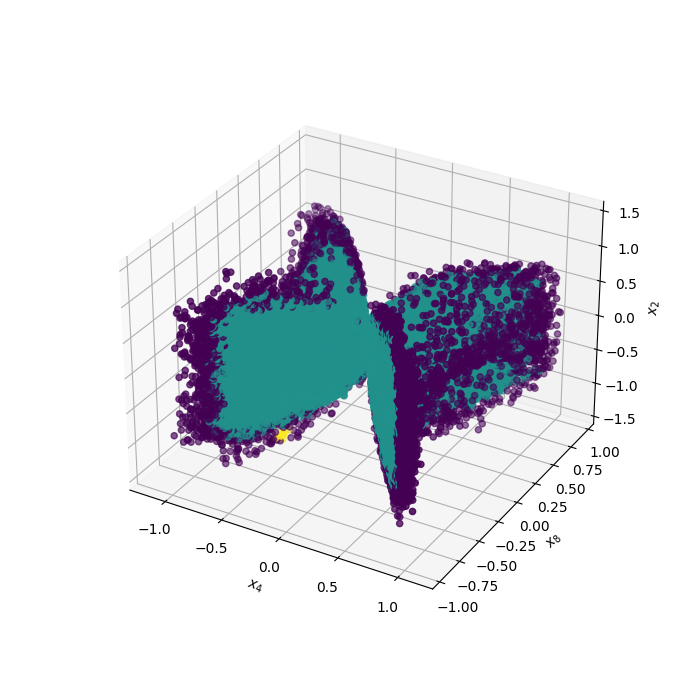
\includegraphics[scale=0.4]{Figures/3d_plot_x2_x4_x8.png}
			\caption{3d plot of $x_4$, $x_8$ and $x_{10}$}
			\label{3dplots}
		\end{figure}
		On these scatter plots, the turquoise points are those belonging to the main cluster, and the purple are those for which the algorithm failed to give them a cluster. On of the two plot, we can see some few yellow points which correspond to the small cluster with 10 points. We can see, from what we can tell with those plots, that all points that could not be assigned to a cluster are on the boarder of the data. Therefore, we interpret the fact that those point could not be assigned, not because there are part of another cluster, and a manifold, but because of the lack of points around them due to the fact they are on the boundary of our data. We conclude from this analysis, that we possess here a sampling of a unique 3 dimensional manifold. 
		
		
		After PCA and clustering we know that the points after the gradient descent sample a three-dimensional manifold.

	\subsection{Annealed Importance Sampling for polynomial symbolic regression}
	\begin{itemize}[label=\textbullet]
		\item We can convert the potential to a polynomial by converting the variables that appear in exponentials to logs.
		\item As the potential is a polynomial, the solutions satisfy polynomials equations. Discuss that fact that we could get polynomials directly by taking the gradient of the potential, but those will be to complicated to express the vacuum in a usable way.  We search those using Annealed Importance Sampling.
		
		Now we have sampled the manifold and exctrated some basic information about it (namely its dimension and the fact that it is made of one block), we would like to see if we can exctract some analytic formula to caracterise it. What we have at the moment, are points on a 3-dimensional manifold, which are embedded in a 5-dimensional space. Therefore we can conclude that, in order to caracterise the manifold, we need two constraints on the embedding coordinates $\vec{x} = (x_1,x_2,x_4,x_8,x_{10})$. If we have a look at the form of the potential \eqref{eq:scalarpotential124810}, we see that if we use $\tilde{x_{8}} = e^{x_8}$, that this potential is actually a polynomial of the embedding coordinates. Therefore, the components of $|\nabla V|$ are also polynomials in those variables. We conclude that the constraints on the embedding coordinates we are looking for are polynomial constraints of the form $p(\vec{x}) = 0$, and that there are two of those. Of course if one takes directly the gradient of \eqref{eq:scalarpotential124810}, one ends up with such conditions, but none are usable directly to solve for two of the variables in terms of the others. The problem we are facing here is therefore a problem of symbolic regression : we are looking for analytic expressions (polynomial) that vanish once evaluated on our data points. There are a number of way one can deal with it, using already existing methods such as AI Feynman methods, or ..., or by doing rough gradient descent on the most general polynomial with arbitrary coefficients and trying to minimize its value once evaluated on the data points. In the spirit of trying to build a generalisable method, we develop here our own method, which is based on symbolic regression using an Annealing Importance Sampling method. 

		\item Annealed Importance Sampling: first explain general idea (construct density probability, role of temperature, links with Monte-Carlo), discuss $\beta$ to control exploration and exploitation phases.
		
		In the realm of symbolic regression, the objective is to uncover interpretable mathematical expressions that best describe a given dataset. In the problem discussed in this paper, we are looking for polynomial expressions such that $p(data) = 0$. This task involves navigating a vast, discrete, and often rugged search space of possible symbolic models, which poses significant challenges for traditional sampling methods. Markov Chain Monte Carlo (MCMC) techniques, while widely used, can struggle with poor mixing and getting trapped in local optima, especially in high-dimensional or multimodal spaces.
		
		To address these challenges, we employ an Annealed Importance Sampling (AIS) combined with Sequential Monte Carlo (SMC) methods. AIS constructs a sequence of intermediate distributions that smoothly transition from an initial, tractable distribution (e.g., a prior over symbolic expressions) to the complex target posterior distribution. This annealing process is guided by a temperature-like parameter that gradually emphasizes the data likelihood, allowing for more efficient exploration of the probability landscape.
		
		SMC enhances this procedure by propagating a population of particles—each representing a candidate symbolic expression—through the sequence of distributions. At each step, particles are reweighted based on the incremental change in the distribution, resampled to focus computational effort on high-probability regions, and mutated via operations. This combination of importance sampling, resampling, and mutation maintains diversity among the particles and prevents premature convergence to suboptimal models.
		
		These features make AIS-SMC particularly well-suited for symbolic regression tasks, where the search space is not only high-dimensional but also structured and discontinuous. 
		
		\item Then more details: discuss hypotheses to compute the weights, choice of transformations, choice of $\beta$, choice of loss, prior, initial sampling, choice of representation for the polynomials.
		
		Let us now explain in more details how does this procedure goes. The goal is to reconstruct some distribution function $p(z)$, where here $z$ in going to be some polynomial. We will try to reconstruct this density function by a serie of density function $\pi_n(z_n) = \gamma_n(z_n)/Z_n$ with $n = 1,\dots,N$ is going to be the number of annealing steps, $\pi_n$ is defined in terms of an unnormalized density $\gamma_n$ and we have the normalizing constant $Z_n = \int \gamma_n(z) \mathrm{dz}$. We also assume we have a sequence of inverse temperature constants $\beta_n$, where $0 = \beta_1 < \beta_2 <\dots< \beta_N = 1$. We then define the unnormalized density at level $n$ in terms of a prior distribution $p_0(z)$ over the hypothesis space and an Loss function $L(z)$
		\begin{equation}
			\gamma_n(z) := p_0(z) \: \exp \left( -\beta_n L(z) \right)
		\end{equation} 
		
		At each step, we have a set of particles $\{z_{n-1}^k, w_{n-1}^k\}$ approximating $\pi_{n-1}$ (meaning $\mathbb{E}_{\pi_{n-1}}[f] \approx \frac{\sum_k w_{n-1}^k f(z_{n-1}^k)}{\sum_k w_{n-1}^k}$), and we want to obtain a new set $\{z_n^k, w_n^k\}$ approximating $\pi_n$. To do so, for each particle $z^k_{n-1}$, we propose a new particle $z_n^k \sim q(z_n | z_{n-1}^k)$ and walculate the new unnormalized importance weight $w_n^k$. 
		
		Let us first focus on how we propose a new particle $z_n^k \sim q(z_n | z_{n-1}^k)$ given $z_{n-1}^k$. To do so, we choose $q(z_n | z_{n-1})$ to be a Markov kernel 
		
		\item Discuss the fact that we allow float coefficients even though we know the coefficients will be only integers of square roots of integers?
		\item Analysis after AIS: select the best polynomials and do exploitation on the coefficients (without MC: we keep only the proposal of it betters the polynomial).
		\item Results for naive choices of parameters (numbers of iteration and particles, probabilities, $\beta$) and motivate them (we want some exploration and then exploitation, not too long computations): for multiple runs we find multiple polynomials (good polynomial: after exploitation we convert the coefficients to integers and square roots, and recompute loss without regularisation, select with threshold). Quantify it nicely: success rates for each polynomials, and absolute number of success, failing rate. Total time needed, without cluster or fancy computers.
	\end{itemize}


	\paragraph{Results}
	We have used the numerical analysis outlined in the previous sections to the search for extrema of the scalar potential~\eqref{eq:scalarpotential124810}. For 100 runs with parameters \ce{\texttt{max degree} is 4, \texttt{max num monomials} is 6.}
	\begin{equation}
		\begin{gathered}
			n_{\rm iter} = 1000, \quad n_{\rm particles} = 1000, \quad {\rm reg} = 10^{3}, \quad \beta = 10^{-10} + \left(\frac{i}{n_{\rm iter}}\right)^{5}, \quad \sigma = 0.5 - \frac{0.45}{1+\exp\big(10-20 i/n_{\rm iter}\big)}, \\
			{\rm sample\ size = 10000},\quad p_{\rm add} = 0, \quad p_{\rm remove} = 0, \quad p_{\rm modify} = 0.5, \quad p_{\rm multiply} = 0.25, \quad p_{\rm divide} = 0.25,
		\end{gathered}
	\end{equation}
	the code finds the 7 different following polynomials: \ce{Mention that we ``rounded'' the coefficients to integer and square root of them.}
	\begin{subequations} \label{eq:pols}
    \begin{align}
      p_{1} &= -\sqrt{2}\,x_{1} + \sqrt{2}\,x_{1}\tilde{x}_{8} + x_{2}\tilde{x}_{8}x_{10} - \sqrt{2}\,x_{2}x_{4}\tilde{x}_{8},\\
      p_{2} &= 2\,x_{2} + 2\,x_{2}\tilde{x}_{8} + \sqrt{2}\,x_{1}x_{10} + 2\,x_{1}x_{4} - x_{2}\tilde{x}_{8}x_{10}^{2},\\
      p_{3} &= 2\,x_{2} - 2\,x_{2}\tilde{x}_{8} + \sqrt{2}\,x_{1}\tilde{x}_{8}x_{10} + 2\,x_{1}x_{4}\tilde{x}_{8}
      		- 2\,x_{2} x_{4}^{2}\tilde{x}_{8},\\
      p_{4} &= \sqrt{2}\,x_{2} - \sqrt{2}\,x_{2}\tilde{x}_{8} + \sqrt{2}\,x_{1}\,x_{4} + x_{1}\tilde{x}_{8}x_{10}
      		- x_{2}x_{4}\tilde{x}_{8}x_{10},\\
      p_{5} &= -2\,x_{1} - 2\,x_{2}x_{4}- 2\,x_{1}x_{4}^{2} + 2\,x_{1}\tilde{x}_{8} + \sqrt{2}\,x_{2}x_{10}
      		+ x_{1}\tilde{x}_{8}x_{10}^{2},\\
      p_{6} &= -2\,x_{2}x_{4} - 2\,x_{1}x_{4}^{2} + 2\,x_{2}x_{4}\tilde{x}_{8} + \sqrt{2}\,x_{2}x_{10} 
      		- \sqrt{2}\,x_{2}\tilde{x}_{8}x_{10} +  x_{1}\tilde{x}_{8}x_{10}^{2},\\
      p_{7} &= -\sqrt{2}\,x_{1}^{2}x_{4} + \sqrt{2}\,x_{2}^{2}x_{4} + \sqrt{2}\,x_{1}x_{2}x_{4}^{2} - x_{1}^{2}x_{10}
      		- x_{2}^{2}x_{10},
    \end{align}
  \end{subequations}
  where $\tilde{x}_{8} = e^{x_{8}}$, with the distribution: \ce{It's not a distribution, how to name it? Frequency?}
  \begin{equation}
  	\begin{tabular}{l|cccccccc}
  		& $p_{1}$ & $p_{2}$ & $p_{3}$ & $p_{4}$ & $p_{5}$ & $p_{6}$ & $p_{7}$ & $\varnothing$ \\\hline\hline
  		Distribution & 59\% & 25\% & 5\% & 9\% & 2\% & 4\% & 2\% & 13\%
  	\end{tabular}
  \end{equation}
  The sum of the percentages is higher than 100\% because some runs find more than one polynomials. The code fails to find any polynomial in 13\% of the time. The averaged time needed for a single run on a PC in $\sim 1400\,{\rm s}$. \ce{This timing is with \texttt{analysis}, it may be less without.}

  \ce{Draw histograms of the polynomials distribution to discuss runs with multiple outputs?}

\section{Supergravity solutions}
\begin{itemize}[label=\textbullet]
	\item For each couple of candidate polynomials, we get the same expression for the solution, and it indeed defines a unique vacuum of the 3d SUGRA.
	\item Discussion of the vacuum: gauge group, Zham. metric, change of variables, 3d spectrum (and stability), spin 2 spectrum on $S^{3}$, one parameter seems to be a gauge parameter, uplift?
\end{itemize}

For every couples $(p_{i},p_{j})$ of polynomials in eq.~\eqref{eq:pols}, the system
\begin{equation}
	\begin{cases}
		p_{i} = 0, \\
		p_{j} = 0,
	\end{cases}
\end{equation}
gives the same solution \ce{That's not true! For example, $x_{1}=x_{2}=0$ solves all polynomials but is not a sugra solution. Mention tests on the sugra?}
\begin{equation}
	\begin{cases}
		\displaystyle x_{1} = \frac{x_{2}}{\sqrt{2}}\,\frac{e^{x_{8}/2}}{e^{x_{8}}-1}\,\Big(-x_{5}\,e^{x_{8}/2} + \sqrt{2-4\,e^{x_{8}}+e^{2x_{8}}\big(2+x_{10}^{2}\big)}\Big),\\[8pt]
		\displaystyle x_{4} = \frac{e^{-x_{8}/2}}{\sqrt{2}}\,\sqrt{2-4\,e^{x_{8}}+e^{2x_{8}}\big(2+x_{10}^{2}\big)}.
	\end{cases}
\end{equation}
We checked that this defines a 3-parameter solution of three-dimensional half-maximal supergravity. Equivalently:
\begin{equation}
	\begin{cases}
		\displaystyle \tilde{x}_{8} = \frac{x_{1}^{2}+x_{2}^{2}}{x_{2}^{2} + \big(x_{1}-x_{2}x_{4}\big)^{2}},\\[10pt]
		\displaystyle x_{10} = \sqrt{2}\,x_{4}\,\frac{x_{2}^{2} - x_{1}^{2}+x_{1}x_{2}x_{4}}{x_{1}^{2}+x_{2}^{2}}.
	\end{cases}
\end{equation}
The solution preserves a ${\rm U}(1)\times{\rm U}(1)$ gauged symmetry.

\paragraph{Moduli space}
The $(x_{1},x_{2},x_{4})$ moduli space is most nicely parametrised using the change of coordinates
\begin{equation}
	x_{1} = r\cos(\theta)\cos(\Phi), \quad x_{2} = r\cos(\theta)\sin(\Phi) \quad {\rm and} \quad x_{4} = r\sin(\theta),
\end{equation}
for which the Zamolodchikov metric reads
\begin{equation}
	\d^{2}s_{\rm Zam.} = -\,\d r^{2} - r^{2}\,\bigg(\d \theta^{2} - r\cos(\theta)\,\d \theta\d\Phi + \sin(\theta)\,\d r\d\Phi + \frac{1}{2}\,\big(3+r^{2}-\cos(2\theta)\big)\,\d\Phi^{2} \bigg).
\end{equation}
\ce{Tests other change of variables? Test choices of variables other than $(x_{1},x_{2},x_{4})$?}

\paragraph{Bosonic spectrum}
Vector fields:
\begin{equation}
 \begin{aligned}	
	m_{\sst{(1)}}\ell_{\rm AdS}:\quad &
	0\ [2],	\quad
	-2\ [5],	\quad
	2\ [1],	\\[5pt]
	&	-1\pm\sqrt{\left(1+r^2\right)^2-2\,r^2\,\cos(2\theta)}\ [2+2],	\\[5pt]
	&	1\pm\sqrt{1+4\,r^2+r^{4}}\ [2+2].
 \end{aligned}
\end{equation}
The integers between square brackets indicate the multiplicity of each eigenvalue. The spectrum includes two massless vectors corresponding to the unbroken ${\rm U}(1)\times {\rm U}(1)$ gauge symmetry, although in three dimensions they are non-propagating.


Scalars:
\begin{equation}
 \begin{aligned}	
	\left(m_{\sst{(0)}}\ell_{\rm AdS}\right)^2:\quad&
	0\ [5],	\quad
	8\ [1],	\quad
	r^{2}\,\left(4+r^2\right)\ [8],	\\[5pt]
	&	2r\,\Big(3\,r+r^{3}\pm(2+r^{2})\,\sqrt{2+r^2-2\,\cos(2\theta)}-r\cos(2\theta)\Big)\ [2+2].
 \end{aligned}
\end{equation}

Gravitini:
\begin{equation}
	m_{{(\nicefrac32)}}\ell_{\rm AdS}:\quad 
	\quad \dfrac1{2}\bigg[1\pm\sqrt{4+2\,r^{2}+r^{4}-2r^{2}\cos(2\theta)}\bigg]\ [4+4],
\end{equation}
no SUSY enhancements other than $r=0$.

No dependence on $\Phi$.

\section{Conclusion}
\begin{itemize}[label=\textbullet]
	\item Conclusion: good prospects of improvement to be able to access higher dimensional cases. Classify flat directions.
	\item Appendix with some details on the code?
\end{itemize}



\bibliography{references}


\end{document}